\subsection{Aproximação geométrica do efetuador em relação à porta de acoplamento}
\label{sec:cap4_app_final_eef}

A aproximação geométrica da ponta da ferramenta em relação à porta de acoplamento foi avaliada a partir da posição do efetuador no referencial da primeira junta ($\{0\}$) e do erro de posição em relação ao alvo no referencial LVLH. A Tabela~\ref{tab:cap4_eef_referencial0_pos} resume as faixas e os valores finais das componentes em $\{0\}$.

\begin{table}[H]
\centering
\caption{Faixas e valores finais da posição do efetuador no referencial da primeira junta ($\{0\}$).}
\label{tab:cap4_eef_referencial0_pos}
\begin{tabularx}{\linewidth}{|
  >{\centering\arraybackslash}X|
  >{\centering\arraybackslash}X|
  >{\centering\arraybackslash}X|}
\hline
\textbf{Componente} &
\textbf{Faixa ao longo da simulação [m]} &
\textbf{Valor final [m]} \\
\hhline{|=|=|=|}
$x_0$ & $0{,}0000 \text{ a } 0{,}1309$ & $0{,}0503$ \\
\hline
$y_0$ & $-0{,}0006 \text{ a } 0{,}8250$ & $-0{,}0006$ \\
\hline
$z_0$ & $0{,}0000 \text{ a } 0{,}9708$ & $0{,}4615$ \\
\hline
\end{tabularx}
\end{table}

\begin{figure}[H]
\centering
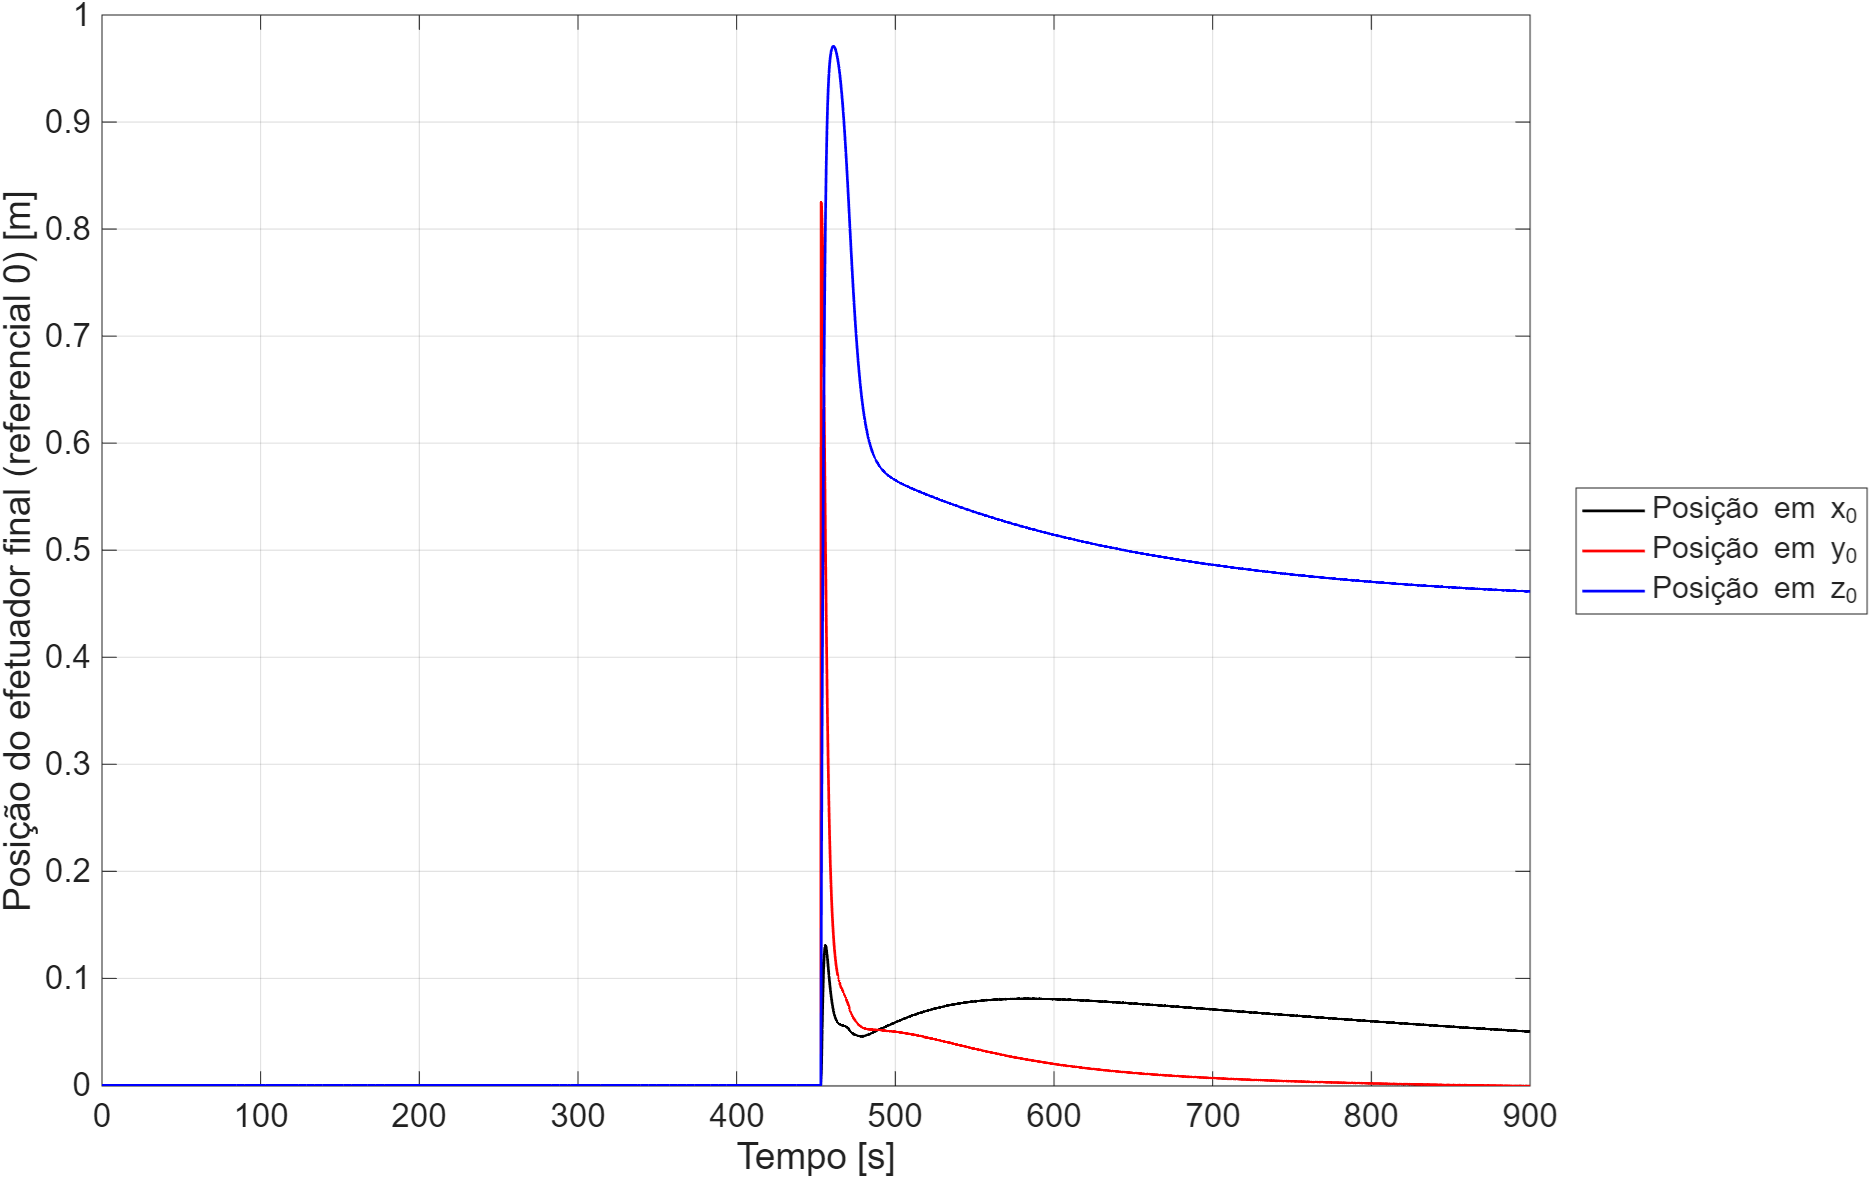
\includegraphics[width=1.0\linewidth]{4 Resultados e discussoes/Imagens/3 App final/8 Posicao eef frame0.png}
\caption{Posição do efetuador final no referencial da primeira junta (referencial 0).}
\label{fig:cap4_app_final_pos_eef_referencial0}
\end{figure}

Por sua vez, a Tabela~\ref{tab:cap4_eef_erro_referencial} apresenta as faixas e os valores finais das componentes de erro $(e_x,e_y,e_z)$, enquanto a Tabela~\ref{tab:cap4_eef_norma_erro} resume a evolução da norma do erro.

\begin{table}[H]
\centering
\caption{Faixas e valores finais das componentes do erro de posição da ferramenta em relação à referência desejada.}
\label{tab:cap4_eef_erro_referencial}
\begin{tabularx}{\linewidth}{|
  >{\centering\arraybackslash}X|
  >{\centering\arraybackslash}X|
  >{\centering\arraybackslash}X|}
\hline
\textbf{Componente} &
\textbf{Faixa ao longo da simulação [m]} &
\textbf{Valor final [m]} \\
\hhline{|=|=|=|}
$e_x$ & $-0{,}0211 \text{ a } 0{,}1142$ & $-0{,}0015$ \\
\hline
$e_y$ & $-0{,}8250 \text{ a } 0{,}0000$ & $-0{,}0045$ \\
\hline
$e_z$ & $-0{,}3848 \text{ a } 0{,}4172$ & $1{,}61\times 10^{-4}$ \\
\hline
\end{tabularx}
\end{table}

\begin{table}[H]
\centering
\caption{Faixa e valor final da norma do erro de posição da ferramenta.}
\label{tab:cap4_eef_norma_erro}
\begin{tabularx}{0.7\linewidth}{|
  >{\centering\arraybackslash}X|
  >{\centering\arraybackslash}X|
  >{\centering\arraybackslash}X|}
\hline
\textbf{Grandeza} &
\textbf{Faixa ao longo da simulação [m]} &
\textbf{Valor final [m]} \\
\hhline{|=|=|=|}
$\|\mathbf{e}\|$ & $0{,}0000 \text{ a } 0{,}9315$ & $0{,}0047$ \\
\hline
\end{tabularx}
\end{table}

\begin{figure}[H]
\centering

\includegraphics[width=1.0\linewidth]{4 Resultados e discussoes/Imagens/3 App final/9 Erro eef.png}
\caption{Erro de posição do efetuador em relação à posição desejada na aproximação final.}
\label{fig:cap4_app_final_erro_eef}
\end{figure}

Os resultados indicam que, ao final da aproximação, o efetuador encontra-se praticamente alinhado em along-track e cross-track (erros de poucos milímetros) e a cerca de $5$ cm da posição alvo na direção radial, com norma do erro em torno de $4{,}7\times 10^{-3}$ m.